\documentclass[tikz,border=10pt]{standalone}
\usepackage{tikz}
\usepackage{fontawesome5}
\usepackage{amsmath,amssymb}
\usetikzlibrary{arrows.meta,positioning,fit,backgrounds,calc,shadows,shapes.geometric}

% Color definitions
\definecolor{lavenderDark}{RGB}{15, 44, 89}
\definecolor{lavenderDeep}{RGB}{10, 28, 58}
\definecolor{lavenderMedium}{RGB}{29, 78, 158}
\definecolor{lavenderLight}{RGB}{240, 246, 255}
\definecolor{lavenderBorder}{RGB}{180, 205, 237}
\definecolor{prismNavy}{RGB}{15, 44, 89}
\definecolor{prismBlue}{RGB}{29, 78, 158}
\definecolor{prismTeal}{RGB}{13, 148, 136}
\definecolor{prismGold}{RGB}{217, 119, 6}
\definecolor{prismDark}{RGB}{15, 23, 42}
\definecolor{statusFail}{RGB}{220, 38, 38}
\definecolor{cInput}{RGB}{241, 245, 249}
\definecolor{cStem}{RGB}{224, 242, 254}
\definecolor{cStage1}{RGB}{209, 250, 229}
\definecolor{cStage2}{RGB}{254, 243, 199}
\definecolor{cStage3}{RGB}{254, 226, 226}
\definecolor{cStage4}{RGB}{207, 250, 254}
\definecolor{cHead}{RGB}{219, 234, 254}

\begin{document}
% Staged Execution Flow & Atomic Double-Voting Mitigation Pipeline
\begin{tikzpicture}[
    x=1cm, y=1cm,
    hdrbox/.style={rectangle, rounded corners=3pt, draw=lavenderDark!60, fill=lavenderDark!12,
      line width=0.7pt, inner sep=4pt, font=\fontsize{8.0}{9.5}\selectfont\bfseries\color{lavenderDark}},
    modelrow/.style={rectangle, rounded corners=3.5pt, draw=lavenderDark!45,
      line width=0.65pt, inner sep=4.5pt},
    arrow/.style={-{Stealth[scale=0.85]}, line width=0.9pt, draw=lavenderDark!85}
]

  % Column Headers
  \node[hdrbox, text width=2.40cm, align=center] at (-5.85, 1.15) {Execution Stage};
  \node[hdrbox, text width=7.40cm, align=center] at (-0.55, 1.15) {On-Chain EVM Validation \& Mutation Logic};
  \node[hdrbox, text width=4.10cm, align=center] at (5.60, 1.15) {Enforced Barrier / Outcome};

  % Stage 1: Caller Whitelist Verification (y = 0.0)
  \node[modelrow, fill=cInput!70, text width=2.40cm, align=center, minimum height=1.20cm] (m1l) at (-5.85, 0.0)
    {{\fontsize{8.5}{10.2}\selectfont\color{lavenderDark}\faUserCheck\ \textbf{1. Whitelist}}\\[3pt]
     {\fontsize{7.5}{9.0}\selectfont\texttt{verifyVoter()}}};
  \node[modelrow, fill=lavenderLight!85, text width=7.40cm, align=left, minimum height=1.20cm] (m1p) at (-0.55, 0.0)
    {\fontsize{7.6}{9.2}\selectfont \textbf{Whitelist Assertion} $\rightarrow$ Check \texttt{voters[msg.sender].isRegistered}\\[2pt]Confirm caller wallet address is certified by administrator};
  \node[modelrow, fill=lavenderLight!85, text width=4.10cm, align=left, minimum height=1.20cm] (m1r) at (5.60, 0.0)
    {\fontsize{7.6}{9.2}\selectfont \textbf{Verified Address}\\[2pt]{\fontsize{6.8}{8.0}\selectfont Revert if unregistered}};

  % Stage 2: Double-Voting Guard (y = -1.75)
  \node[modelrow, fill=cStage3!65, text width=2.40cm, align=center, minimum height=1.20cm] (m2l) at (-5.85, -1.75)
    {{\fontsize{8.5}{10.2}\selectfont\color{statusFail!90!black}\faBan\ \textbf{2. Anti-Replay}}\\[3pt]
     {\fontsize{7.5}{9.0}\selectfont\texttt{doubleVoteGuard}}};
  \node[modelrow, fill=lavenderLight!85, text width=7.40cm, align=left, minimum height=1.20cm] (m2p) at (-0.55, -1.75)
    {\fontsize{7.6}{9.2}\selectfont \textbf{Double-Voting Condition} $\rightarrow$ Check \texttt{!voters[msg.sender].hasVoted}\\[2pt]Atomic predicate verification: $\text{Accept}(v) \iff \neg\text{voted}(v)$};
  \node[modelrow, fill=lavenderLight!85, text width=4.10cm, align=left, minimum height=1.20cm] (m2r) at (5.60, -1.75)
    {\fontsize{7.6}{9.2}\selectfont \textbf{Single-Ballot Guard}\\[2pt]{\fontsize{6.8}{8.0}\selectfont Revert if already cast}};

  % Stage 3: Candidate Range Verification (y = -3.50)
  \node[modelrow, fill=cStage2!65, text width=2.40cm, align=center, minimum height=1.20cm] (m3l) at (-5.85, -3.50)
    {{\fontsize{8.5}{10.2}\selectfont\color{prismGold!90!black}\faVoteYea\ \textbf{3. Ballot Audit}}\\[3pt]
     {\fontsize{7.5}{9.0}\selectfont\texttt{candidateCheck}}};
  \node[modelrow, fill=lavenderLight!85, text width=7.40cm, align=left, minimum height=1.20cm] (m3p) at (-0.55, -3.50)
    {\fontsize{7.6}{9.2}\selectfont \textbf{Range Verification} $\rightarrow$ Assert $c \in [1, \text{candidatesCount}]$\\[2pt]Prevent out-of-bounds index access and fabricated candidates};
  \node[modelrow, fill=lavenderLight!85, text width=4.10cm, align=left, minimum height=1.20cm] (m3r) at (5.60, -3.50)
    {\fontsize{7.6}{9.2}\selectfont \textbf{Certified Candidate}\\[2pt]{\fontsize{6.8}{8.0}\selectfont Revert on invalid $c$}};

  % Stage 4: Atomic State Mutation (y = -5.25)
  \node[modelrow, fill=cStage1!65, text width=2.40cm, align=center, minimum height=1.20cm] (m4l) at (-5.85, -5.25)
    {{\fontsize{8.5}{10.2}\selectfont\color{prismTeal!90!black}\faSave\ \textbf{4. State Mutate}}\\[3pt]
     {\fontsize{7.5}{9.0}\selectfont\texttt{atomicCommit()}}};
  \node[modelrow, fill=lavenderLight!85, text width=7.40cm, align=left, minimum height=1.20cm] (m4p) at (-0.55, -5.25)
    {\fontsize{7.6}{9.2}\selectfont \textbf{Single-Transaction Mutation} $\rightarrow$ \texttt{voters[msg.sender].hasVoted = true}\\[2pt]Atomic ledger mutation: Increment tally $N(c) \leftarrow N(c) + 1$};
  \node[modelrow, fill=lavenderLight!85, text width=4.10cm, align=left, minimum height=1.20cm] (m4r) at (5.60, -5.25)
    {\fontsize{7.6}{9.2}\selectfont \textbf{State Trie Updated}\\[2pt]{\fontsize{6.8}{8.0}\selectfont Nonce consumed}};

  % Stage 5: Event Emission & Consensus (y = -7.00)
  \node[modelrow, fill=cHead!65, text width=2.40cm, align=center, minimum height=1.20cm] (m5l) at (-5.85, -7.00)
    {{\fontsize{8.5}{10.2}\selectfont\color{prismNavy}\faCube\ \textbf{5. Block Seal}}\\[3pt]
     {\fontsize{7.5}{9.0}\selectfont\texttt{PoAConsensus}}};
  \node[modelrow, fill=lavenderLight!85, text width=7.40cm, align=left, minimum height=1.20cm] (m5p) at (-0.55, -7.00)
    {\fontsize{7.6}{9.2}\selectfont \textbf{Event Emission} $\rightarrow$ \texttt{emit VoteCast(msg.sender, c, time)}\\[2pt]Transaction batched into Block $B_i$ and broadcast to validator network};
  \node[modelrow, fill=lavenderLight!85, text width=4.10cm, align=left, minimum height=1.20cm] (m5r) at (5.60, -7.00)
    {\fontsize{7.6}{9.2}\selectfont \textbf{Immutable Receipt}\\[2pt]{\fontsize{6.8}{8.0}\selectfont Broadcast to Web3 UI}};

  % Horizontal assertion flow across each stage
  \draw[arrow] (m1l) -- (m1p);
  \draw[arrow] (m1p) -- (m1r);

  \draw[arrow] (m2l) -- (m2p);
  \draw[arrow] (m2p) -- (m2r);

  \draw[arrow] (m3l) -- (m3p);
  \draw[arrow] (m3p) -- (m3r);

  \draw[arrow] (m4l) -- (m4p);
  \draw[arrow] (m4p) -- (m4r);

  \draw[arrow] (m5l) -- (m5p);
  \draw[arrow] (m5p) -- (m5r);

  % Vertical pipeline execution flow down stages
  \draw[arrow, line width=1.1pt, draw=lavenderDark, shorten <=3pt, shorten >=4.5pt] (m1l) -- (m2l);
  \draw[arrow, line width=1.1pt, draw=lavenderDark, shorten <=3pt, shorten >=4.5pt] (m2l) -- (m3l);
  \draw[arrow, line width=1.1pt, draw=lavenderDark, shorten <=3pt, shorten >=4.5pt] (m3l) -- (m4l);
  \draw[arrow, line width=1.1pt, draw=lavenderDark, shorten <=3pt, shorten >=4.5pt] (m4l) -- (m5l);

\end{tikzpicture}
\end{document}
